\chapter{A4}

{\LARGE 'What are the top 50 most popular applications used by the computers in the domain?'}

\textbf{Nota:} There is a Wikipedia page that lists the assigned port numbers, https://en.wikipedia.org/wiki/List\_of\_TCP\_and\_UDP\_port\_numbers. Or you can Google for the IANA’s Well Known Port Numbers.

\section{Explicação do código desenvolvido}

A computação deste tópico já trouxe mais dificuldades, não propriamente no conseguir os resultados, mas em trata-los de forma a ter um output compreensível e legível. No excerto de código abaixo, mostramos que fomos simplesmente buscar os dados que nos interessavam, ou seja \textit{Source Port, Destination Port e Packets}, às colunas correspondentes do ficheiro bigFlows.csv.

\begin{figure}[h!]
    \label{high}
    \centering
    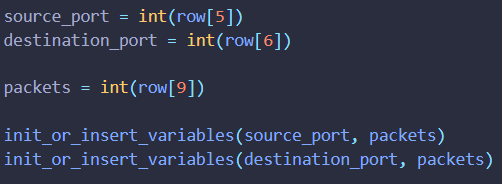
\includegraphics[width=0.9\textwidth]{Images/a4/a4.png}
    \caption{\textit{Código do tópico a4}}
\end{figure}

\newpage

É neste excerto de código que fazemos o tratamento de dados de forma semelhante aos tópicos anteriores.

\begin{figure}[h!]
    \label{high}
    \centering
    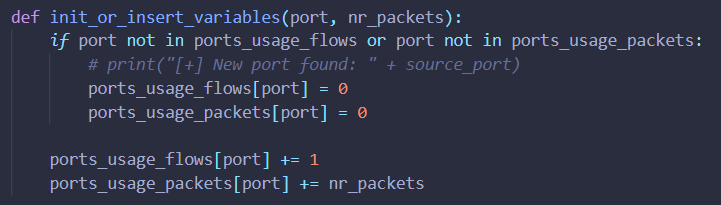
\includegraphics[width=0.9\textwidth]{Images/a4/initOrInsertVariables.png}
    \caption{\textit{Código auxiliar do tópico a4}}
\end{figure}

E para termos um output compreensível usamos as seguintes funções auxiliares. A primeira dá-nos um mapa onde cada por corresponde um uma aplicação, como exemplo temos o \textit{port 80} que corresponde a \textit{Hypertext Transfer Protocol (http)}. A segunda "pega" nos ports dos nossos resultados e atribui-lhes um nome baseado nesse mapa, como exemplo se tivermos um \textit{port 443} nos nossos resultados, esta função atribui-lhe o nome https como está no mapa.

\begin{figure}[h!]
    \label{high}
    \centering
    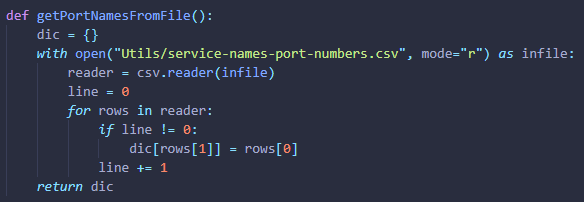
\includegraphics[width=0.9\textwidth]{Images/a4/getPortNamesFromFile.png}
    \caption{\textit{Código auxiliar do tópico a4}}
\end{figure}

\begin{figure}[h!]
    \label{high}
    \centering
    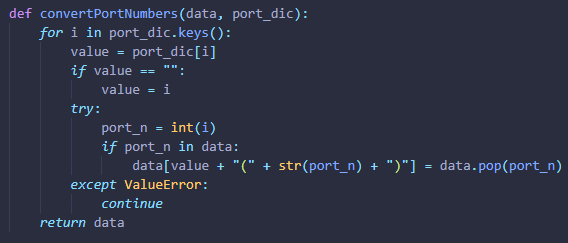
\includegraphics[width=0.9\textwidth]{Images/a4/convertPortNumbers.png}
    \caption{\textit{Código auxiliar do tópico a4}}
\end{figure}

\newpage


\section{Resultados obtidos pelo ficheiro bigFlows.csv}

No enunciado do trabalho é nos perguntado se somos surpreendidos pelo resultado. A resposta é sim e não. Foi surpreendente a quantidade de ports que obtivemos que não tiveram nenhum mapeamento aos ports da lista que usamos, sendo que nem todos são de aplicações externas (ports 49152 a 65535). No entanto, dos ports que conseguimos identificar, já esperávamos quais é que teriam mais fluxo.

\begin{figure}[h]
    \label{high}
    \centering
    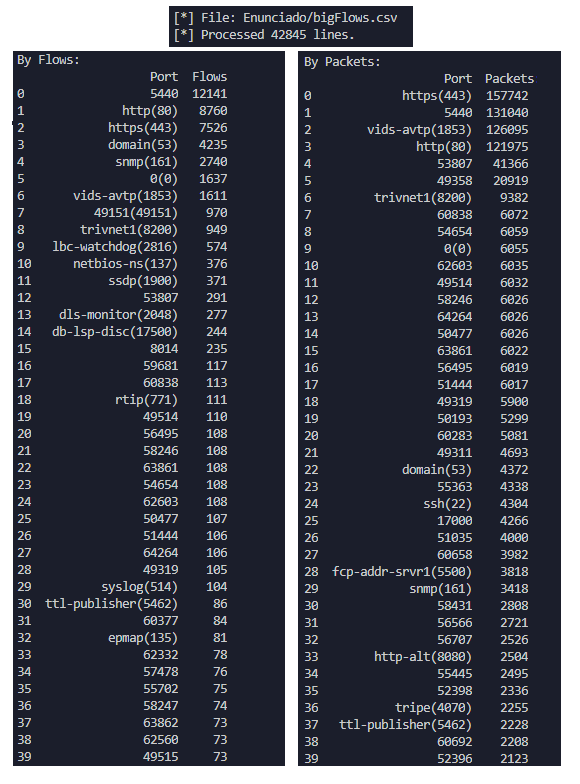
\includegraphics[width=0.85\textwidth]{Images/a4/a4_a.png}
    \caption{\textit{Output do script a4.py}}
\end{figure}

